\documentclass[12pt]{article}

\usepackage{sbc-template}
\usepackage{graphicx,url}
\usepackage[utf8]{inputenc}
\usepackage[T1]{fontenc}
\usepackage[brazil]{babel}
\usepackage{booktabs}
\usepackage{tabularx}
\usepackage{array}
\usepackage{microtype}
\usepackage{placeins}

\sloppy

\title{Análise Experimental de TCP CUBIC, BBR e 0-RTT QUIC em Rede Emulada}

\author{[NOME COMPLETO DO(A) DISCENTE]\inst{1}}

\address{Universidade Federal do Piauí (UFPI)\\
  Terceira Avaliação de Redes de Computadores II
  \email{[E-MAIL ACADÊMICO]}
}

\begin{document}

\maketitle

\begin{abstract}
This paper experimentally evaluates TCP CUBIC and BBR under emulated delay and loss, and compares the time to first byte of HTTP/2, cold HTTP/3, and resumed HTTP/3 with accepted 0-RTT data. Thirty audited measurements were collected in a Docker Desktop/WSL2 environment using \texttt{iperf3}, \texttt{curl}, Caddy, and \texttt{tc netem}. Under 50~ms RTT and 2\% loss, BBR achieved 70.57 times the mean throughput of CUBIC. With 50~ms RTT and no induced loss, HTTP/3 0-RTT reduced mean TTFB by 64.35\% relative to HTTP/2. The results explain mechanisms observed in this setup and are not claims of universal superiority.
\end{abstract}

\begin{resumo}
Este artigo avalia experimentalmente TCP CUBIC e BBR sob atraso e perda emulados e compara o tempo até o primeiro byte de HTTP/2, HTTP/3 sem sessão prévia e HTTP/3 retomado com dados 0-RTT aceitos. Trinta medições auditadas foram obtidas em Docker Desktop/WSL2 com \texttt{iperf3}, \texttt{curl}, Caddy e \texttt{tc netem}. Com RTT de 50~ms e perda de 2\%, BBR alcançou vazão média 70,57 vezes maior que CUBIC. Com RTT de 50~ms e sem perda induzida, HTTP/3 0-RTT reduziu o TTFB médio em 64,35\% frente ao HTTP/2. Os resultados explicam os mecanismos observados neste ambiente, sem afirmar superioridade universal.\\
\textbf{Palavras-chave:} controle de congestionamento; CUBIC; BBR; QUIC; HTTP/3; 0-RTT.
\end{resumo}

\section{Introdução}

O desempenho de aplicações em rede depende tanto da capacidade do caminho quanto da forma como o transporte reage a atraso, perdas e estabelecimento de conexões. Algoritmos de controle de congestionamento regulam a quantidade de dados em trânsito para utilizar a rede sem provocar colapso. CUBIC, amplamente empregado em TCP, usa uma função cúbica para reconstruir a janela de congestionamento após eventos de perda \cite{rfc9438}. BBR segue outra abordagem: estima a largura de banda do gargalo e o menor RTT observado para construir um modelo do caminho \cite{cardwell2016bbr}. Em redes onde descartes não representam saturação, essas estratégias podem produzir comportamentos distintos.

Também há custos antes da transferência. HTTP/2 normalmente combina TCP e TLS, enquanto HTTP/3 utiliza QUIC sobre UDP e integra o estabelecimento do transporte ao TLS~1.3 \cite{rfc9000,rfc9001,rfc9114}. Com estado criptográfico obtido anteriormente, session resumption e 0-RTT permitem enviar dados de aplicação no primeiro voo, embora com restrições de segurança, como risco de replay \cite{rfc8446}.

Este trabalho investiga dois problemas. O Bloco~A mede o impacto de uma WAN degradada na vazão e nas retransmissões de TCP CUBIC e compara CUBIC e BBR sob o mesmo perfil. O Bloco~B compara o TTFB de HTTP/2, HTTP/3 em conexão nova (\emph{Cold}) e HTTP/3 em nova conexão com retomada e 0-RTT aceito. A contribuição é uma análise mecanística e reproduzível de 30 medições oficiais, acompanhada de limitações que delimitam sua validade externa.

\section{Fundamentação Teórica}

\subsection{TCP CUBIC e TCP BBR}

CUBIC é orientado por perdas: após um evento de congestionamento, reduz multiplicativamente \texttt{cwnd}, preserva uma referência da janela anterior e volta a aumentá-la em função do tempo desde o evento. O perfil cúbico cresce de forma côncava ao se aproximar da janela anterior, permanece menos agressivo nas proximidades desse ponto e depois assume perfil convexo \cite{rfc9438}. Perdas recorrentes reduzem o volume em voo; RTT maior alonga o ciclo entre envio, reconhecimento e recuperação. Assim, perdas aleatórias combinadas a RTT elevado podem manter a janela abaixo do necessário para ocupar o caminho.

BBR estima \emph{Bottleneck Bandwidth} e \emph{Round-trip propagation time}. O produto entre largura de banda e RTT mínimo aproxima o \emph{Bandwidth-Delay Product} (BDP), isto é, o volume que pode ocupar o caminho. A partir do modelo, BBR controla dados em voo e ritmo de envio (\emph{pacing}) para operar próximo desse ponto, sem usar toda perda como sinal primário de redução \cite{cardwell2016bbr}. Isso pode preservar vazão quando a perda não corresponde a congestionamento, mas não garante superioridade: filas, competição, versão do algoritmo, pacing e características do gargalo afetam o resultado.

\subsection{QUIC, retomada e 0-RTT}

QUIC transporta pacotes em datagramas UDP, oferece fluxos e incorpora TLS~1.3 ao handshake de transporte \cite{rfc9000,rfc9001}. HTTP/3 mapeia a semântica HTTP sobre esses fluxos \cite{rfc9114}. Uma conexão \emph{Cold} ainda precisa negociar chaves e parâmetros; ela não equivale a reutilizar uma conexão existente. Na retomada, um ticket emitido após sessão anterior permite negociar uma PSK na nova conexão. Se o servidor autorizar 0-RTT, a requisição pode seguir como \emph{early data} antes de terminar o handshake \cite{rfc8446}. Portanto, reutilização de conexão, retomada de sessão e 0-RTT aceito são mecanismos diferentes e exigem evidências próprias.

O enunciado indica as Seções 6.5.11, 6.6.2 e 6.6.1 da 6ª edição de Tanenbaum. Como o texto integral e os dados bibliográficos dessa edição não estavam disponíveis no workspace, não foram atribuídos trechos ou páginas ao livro. A fundamentação usa fontes primárias verificáveis; a referência ao livro deve ser conferida e inserida antes da entrega.

\section{Metodologia Experimental}

Os ensaios foram executados no Windows~11 com Docker Desktop/WSL2 e kernel Linux compartilhado. A bridge \texttt{net\_bench} conectou \texttt{client-bench} (172.20.0.50), \texttt{server-tcp} (172.20.0.10, \texttt{iperf3}) e \texttt{server-http3} (172.20.0.30, Caddy com TLS~1.3, HTTP/2 e HTTP/3). O cliente reuniu \texttt{iperf3} e \texttt{curl} com HTTP/2, HTTP/3 e exportação de sessões. A seleção real de CUBIC ou BBR foi confirmada no socket TCP, não apenas solicitada na linha de comando.

\texttt{tc netem} aplicou três perfis: LAN, com RTT alvo de 1~ms e perda zero; WAN degradada, com RTT de 50~ms e perda estocástica de 2\% no sentido dos dados TCP; e WAN sem perda, com RTT de 50~ms. O atraso foi dividido entre cliente e servidor. As qdiscs eram limpas e reaplicadas entre amostras, e os RTTs foram verificados. Não se adicionou \texttt{sch\_fq} nem limite explícito de banda.

E01 mediu CUBIC na LAN; E02, CUBIC na WAN degradada; E03, BBR no mesmo perfil degradado. Cada execução usou uma conexão TCP cliente--servidor por 15~s e registrou vazão do transmissor e retransmissões. E04 mediu HTTP/2, E05 HTTP/3 Cold e E06 HTTP/3 retomado com 0-RTT, todos na WAN sem perda. O objeto possuía 1.024 bytes e o TTFB foi obtido de \texttt{time\_starttransfer}. Em E06, processos e portas UDP distintos provaram nova conexão; o trace confirmou retomada, 84 bytes de \emph{early data} e o Caddy confirmou a aceitação. Logo, o mecanismo não foi inferido apenas pela latência.

Foram coletadas cinco amostras válidas por experimento. Calcularam-se média, mediana, extremos, coeficiente de variação e desvio-padrão amostral $s$ com denominador $n-1$. As barras de erro representam $s$, não erro-padrão ou intervalo de confiança. Não foram realizados testes de hipótese.

\begin{table}[!ht]
\centering
\caption{Resumo das 30 medições oficiais; $s$ é o desvio-padrão amostral.}
\label{tab:resultados}
\small
\begin{tabularx}{\textwidth}{@{}c>{\raggedright\arraybackslash}X>{\raggedright\arraybackslash}Xr@{}}
\toprule
ID & Configuração e cenário & Média $\pm s$ & Retrans. \\
\midrule
E01 & CUBIC; 1 ms; 0\% & $24\,685{,}5634 \pm 67{,}5367$ Mbps & 0 \\
E02 & CUBIC; 50 ms; 2\% & $4{,}1240 \pm 0{,}6387$ Mbps & 400 \\
E03 & BBR; 50 ms; 2\% & $291{,}0168 \pm 8{,}9203$ Mbps & 37.832 \\
E04 & HTTP/2; 50 ms; 0\% & $158{,}9658 \pm 0{,}3345$ ms & -- \\
E05 & HTTP/3 Cold; 50 ms; 0\% & $109{,}4652 \pm 1{,}3737$ ms & -- \\
E06 & HTTP/3 0-RTT; 50 ms; 0\% & $56{,}6664 \pm 0{,}5518$ ms & -- \\
\bottomrule
\end{tabularx}
\end{table}

\section{Resultados e Discussão}

\subsection{CUBIC e BBR}

A Figura~\ref{fig:tcp} apresenta as médias do Bloco~A. O painel logarítmico mantém visíveis as quatro ordens de grandeza entre os casos, enquanto o painel linear amplia a comparação WAN sem omitir E01. Ao passar da LAN para a WAN degradada, CUBIC caiu de 24.685,5634 para 4,1240~Mbps: redução de 24.681,4394~Mbps (99,9833\%) e razão E01/E02 de 5.985,85. Como RTT e perda mudaram simultaneamente, esse contraste não identifica o efeito causal de cada variável. Ele é, contudo, coerente com ciclos de realimentação mais longos e sucessivas reduções de \texttt{cwnd} diante de perda.

\begin{figure}[!t]
\centering
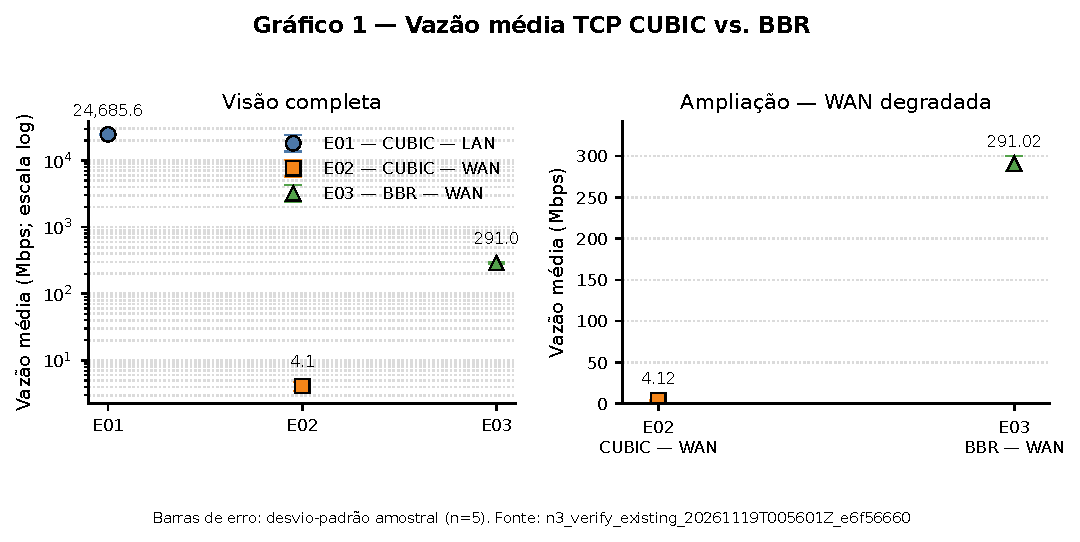
\includegraphics[width=.96\textwidth]{../../results/figures/graph_01_tcp_throughput.pdf}
\caption{Vazão de E01--E03 (média $\pm$ desvio-padrão amostral; $n=5$).}
\label{fig:tcp}
\end{figure}

Sob o mesmo perfil WAN, BBR atingiu 291,0168~Mbps, ganho de 286,8928~Mbps sobre CUBIC, ou 6.956,69\%; a razão BBR/CUBIC foi 70,57. O coeficiente de variação também caiu de 15,49\% para 3,07\%. A observação é compatível com o modelo de banda e RTT mínimo do BBR, menos dependente de interpretar descarte aleatório como saturação. Não demonstra, entretanto, que BBR prevalecerá em outros gargalos.

E03 registrou 37.832 retransmissões, contra 400 em E02. A contagem absoluta não é taxa de perda: em tempo fixo, E03 enviou 2.728.525.824 bytes e E02 apenas 38.666.240 bytes. A normalização descritiva resulta em 13.865,36 e 10.344,94 retransmissões por GB decimal, respectivamente, mas ainda não mede bytes únicos perdidos ou segmentos originais. Portanto, maior retransmissão absoluta não contradiz a maior vazão, nem basta para avaliar eficiência.

\subsection{HTTP/2, HTTP/3 Cold e 0-RTT}

A Figura~\ref{fig:http} mostra queda progressiva do TTFB. HTTP/3 Cold alcançou 109,4652~ms, 49,5006~ms (31,14\%) abaixo dos 158,9658~ms de HTTP/2. No arranjo medido, HTTP/2 paga o estabelecimento TCP e a negociação TLS antes da requisição; QUIC combina negociação criptográfica e transporte, reduzindo dependências sequenciais. A diferença próxima ao RTT alvo é compatível com essa economia, mas também inclui particularidades de Caddy, curl e da bridge virtual.

\begin{figure}[!t]
\centering
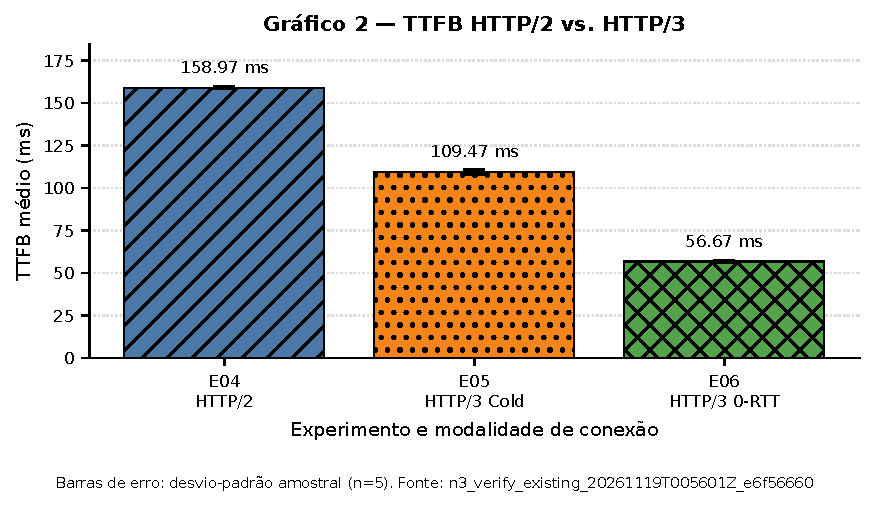
\includegraphics[width=.80\textwidth]{../../results/figures/graph_02_http_ttfb.pdf}
\caption{TTFB de E04--E06 (média $\pm$ desvio-padrão amostral; $n=5$).}
\label{fig:http}
\end{figure}

Com retomada e 0-RTT aceito, E06 obteve 56,6664~ms: redução de 102,2994~ms (64,35\%) frente a E04 e de 52,7988~ms (48,23\%) frente a E05. O ganho E05--E06 também se aproxima de um RTT porque a requisição foi antecipada no primeiro voo. Essa proximidade não prova 0-RTT; a conclusão depende das evidências independentes de ticket, processo, porta, trace, bytes antecipados e aceitação pelo servidor. O resultado vale para um GET idempotente de 1.024 bytes; 0-RTT exige cautela com operações sujeitas a replay.

\FloatBarrier
\section{Limitações Experimentais}

Cinco repetições descrevem dispersão, sem inferência de significância. Docker Desktop/WSL2, bridge e kernel compartilhado limitam a generalização. Não houve gargalo explícito; perda estocástica de \texttt{netem} e qdisc sem \texttt{sch\_fq} podem interagir com pacing. E01/E02 altera atraso e perda simultaneamente, e versões de kernel, Caddy, curl e BBR condicionam os resultados. Perfis auditados e a igualdade E02/E03 sustentam validade interna, não extrapolação.

\section{Conclusão}

Na WAN com 50~ms e 2\% de perda, CUBIC perdeu quase toda a vazão da LAN; BBR atingiu 70,57 vezes a vazão de CUBIC, compatível com seu modelo, mas com muitas retransmissões e sem implicar superioridade universal. HTTP/3 Cold reduziu o TTFB em 31,14\% frente a HTTP/2, e QUIC retomado com 0-RTT aceito reduziu-o em 64,35\%. Evidências de protocolo comprovaram o mecanismo. Os objetivos foram atendidos sob as limitações de amostragem, virtualização, fila e topologia.

\bibliographystyle{sbc}
\bibliography{references}

\end{document}
